\documentclass[conference]{IEEEtran}
% SearchBridge AI -- CSD358 Information Retrieval course project report.
% Structure follows the course brief: Title, Abstract, Introduction, Literature Review, Objective,
% Proposed Model, Methodology, Experimentation and Results, Conclusions and Limitations, References.
% Compile with pdfLaTeX (e.g. upload this folder to Overleaf).
\IEEEoverridecommandlockouts
\usepackage{cite}
\usepackage{amsmath,amssymb}
\usepackage{graphicx}
\usepackage{booktabs}
\usepackage{array}
\usepackage{multirow}
\usepackage{xcolor}
\usepackage{tikz}
\usetikzlibrary{positioning,arrows.meta,fit}
\usepackage{url}
\usepackage[hidelinks]{hyperref}
\graphicspath{{figures/}}

\begin{document}

\title{SearchBridge: An Explainable Hybrid Search Engine}

\author{\IEEEauthorblockN{Aaditya Kharkia}
\IEEEauthorblockA{\textit{Shiv Nadar University}\\
Greater Noida, India\\
Roll no. 2410110492\\
ak897@snu.edu.in}
\and
\IEEEauthorblockN{Preksha Chavan}
\IEEEauthorblockA{\textit{Shiv Nadar University}\\
Greater Noida, India\\
Roll no. 2410110590\\
pc782@snu.edu.in}
\and
\IEEEauthorblockN{Aditya Chauhan}
\IEEEauthorblockA{\textit{Shiv Nadar University}\\
Greater Noida, India\\
Roll no. 2410110504\\
ac830@snu.edu.in}
}

\maketitle

\begin{abstract}
Keyword search misses documents that use different words, while purely semantic search misses exact terms, and neither tells the user why a result was chosen. We present SearchBridge AI, a complete, explainable search engine built for the CSD358 Information Retrieval course. It implements the full syllabus in one running system: text pre-processing, a compressed positional inverted index, Boolean and ranked retrieval (vector space, BM25, language models, a Markov random field model), a polite web crawler, three versions of PageRank and HITS, Naive Bayes and vector-space classifiers, flat and hierarchical clustering, and relevance feedback. On top of these it adds semantic and hybrid retrieval, query expansion and reformulation, context-aware retrieval, query suggestions, near-duplicate detection, personalized retrieval and per-result explanations. Our main method, Bridge-PRF, feeds one hybrid feedback set back into both the lexical and the semantic retriever. On the Cranfield test collection it reaches a mean average precision (MAP) of 0.386, 22\% above BM25 (0.317, $p<0.05$), and higher than our re-implementations of reciprocal-rank fusion, RM3 and dense pseudo-relevance feedback from the literature. On a 21,000-paper sample of the DBLP citation network that we built (165,793 citations), Naive Bayes classifies papers into six fields with 89.6\% accuracy and 0.895 macro-F1, and 96.9\% accuracy on BBC News. We also report what did not work, and show that testing the deployed system against ground truth found eight defects whose fixes raised its precision at 10 by about 6\%.
\end{abstract}

\begin{IEEEkeywords}
information retrieval, BM25, hybrid retrieval, pseudo-relevance feedback, PageRank, HITS, text classification, clustering, explainable ranking
\end{IEEEkeywords}

%=====================================================================
\section{Introduction}
\subsection{Background}
An information retrieval (IR) system finds, in a large collection, the documents that satisfy an information need expressed as a short query~\cite{manning2008}. Modern search engines combine many techniques: an inverted index for speed, a ranking function such as BM25~\cite{robertson2009}, link analysis such as PageRank~\cite{brin1998}, classification and clustering to organise results, and feedback to refine the query~\cite{rocchio1971}. In the last few years, dense sentence embeddings~\cite{reimers2019} have added the ability to match meaning rather than words.

\subsection{Importance and Motivation}
Each family of techniques fails in a different way. Lexical models miss relevant documents that use other words (vocabulary mismatch); semantic models drift away from exact, rare terms; link analysis rewards popular documents whether or not they answer the query; and almost no system explains its ranking to the user. Students, researchers and readers of news all face these problems daily when searching papers or articles. Our motivation was to build one system that combines the strengths of these techniques, explains every result, and is measured honestly component by component, so that it is both useful and a faithful demonstration of the IR syllabus.

\subsection{Contributions}
\begin{itemize}
\item \textbf{A complete search engine} implementing all 17 syllabus topics and 10 advanced features (Table~\ref{tab:syllabus}), with a web interface and per-result explanations (Fig.~\ref{fig:ui}).
\item \textbf{Bridge-PRF}, a hybrid pseudo-relevance feedback method that improves MAP by 22\% over BM25 on Cranfield, with an ablation that shows which of its parts matter.
\item \textbf{Collection-relative gating} of context and link evidence, which switches these signals on only when the data supports them.
\item \textbf{A new evaluation dataset}: a densely linked, labelled 21,000-paper sample of the 4.9-million-paper DBLP citation network.
\item \textbf{Honest negative results} and a \textbf{ground-truth testing method} that found eight defects in the deployed system.
\end{itemize}

\begin{figure*}[t]
\centering
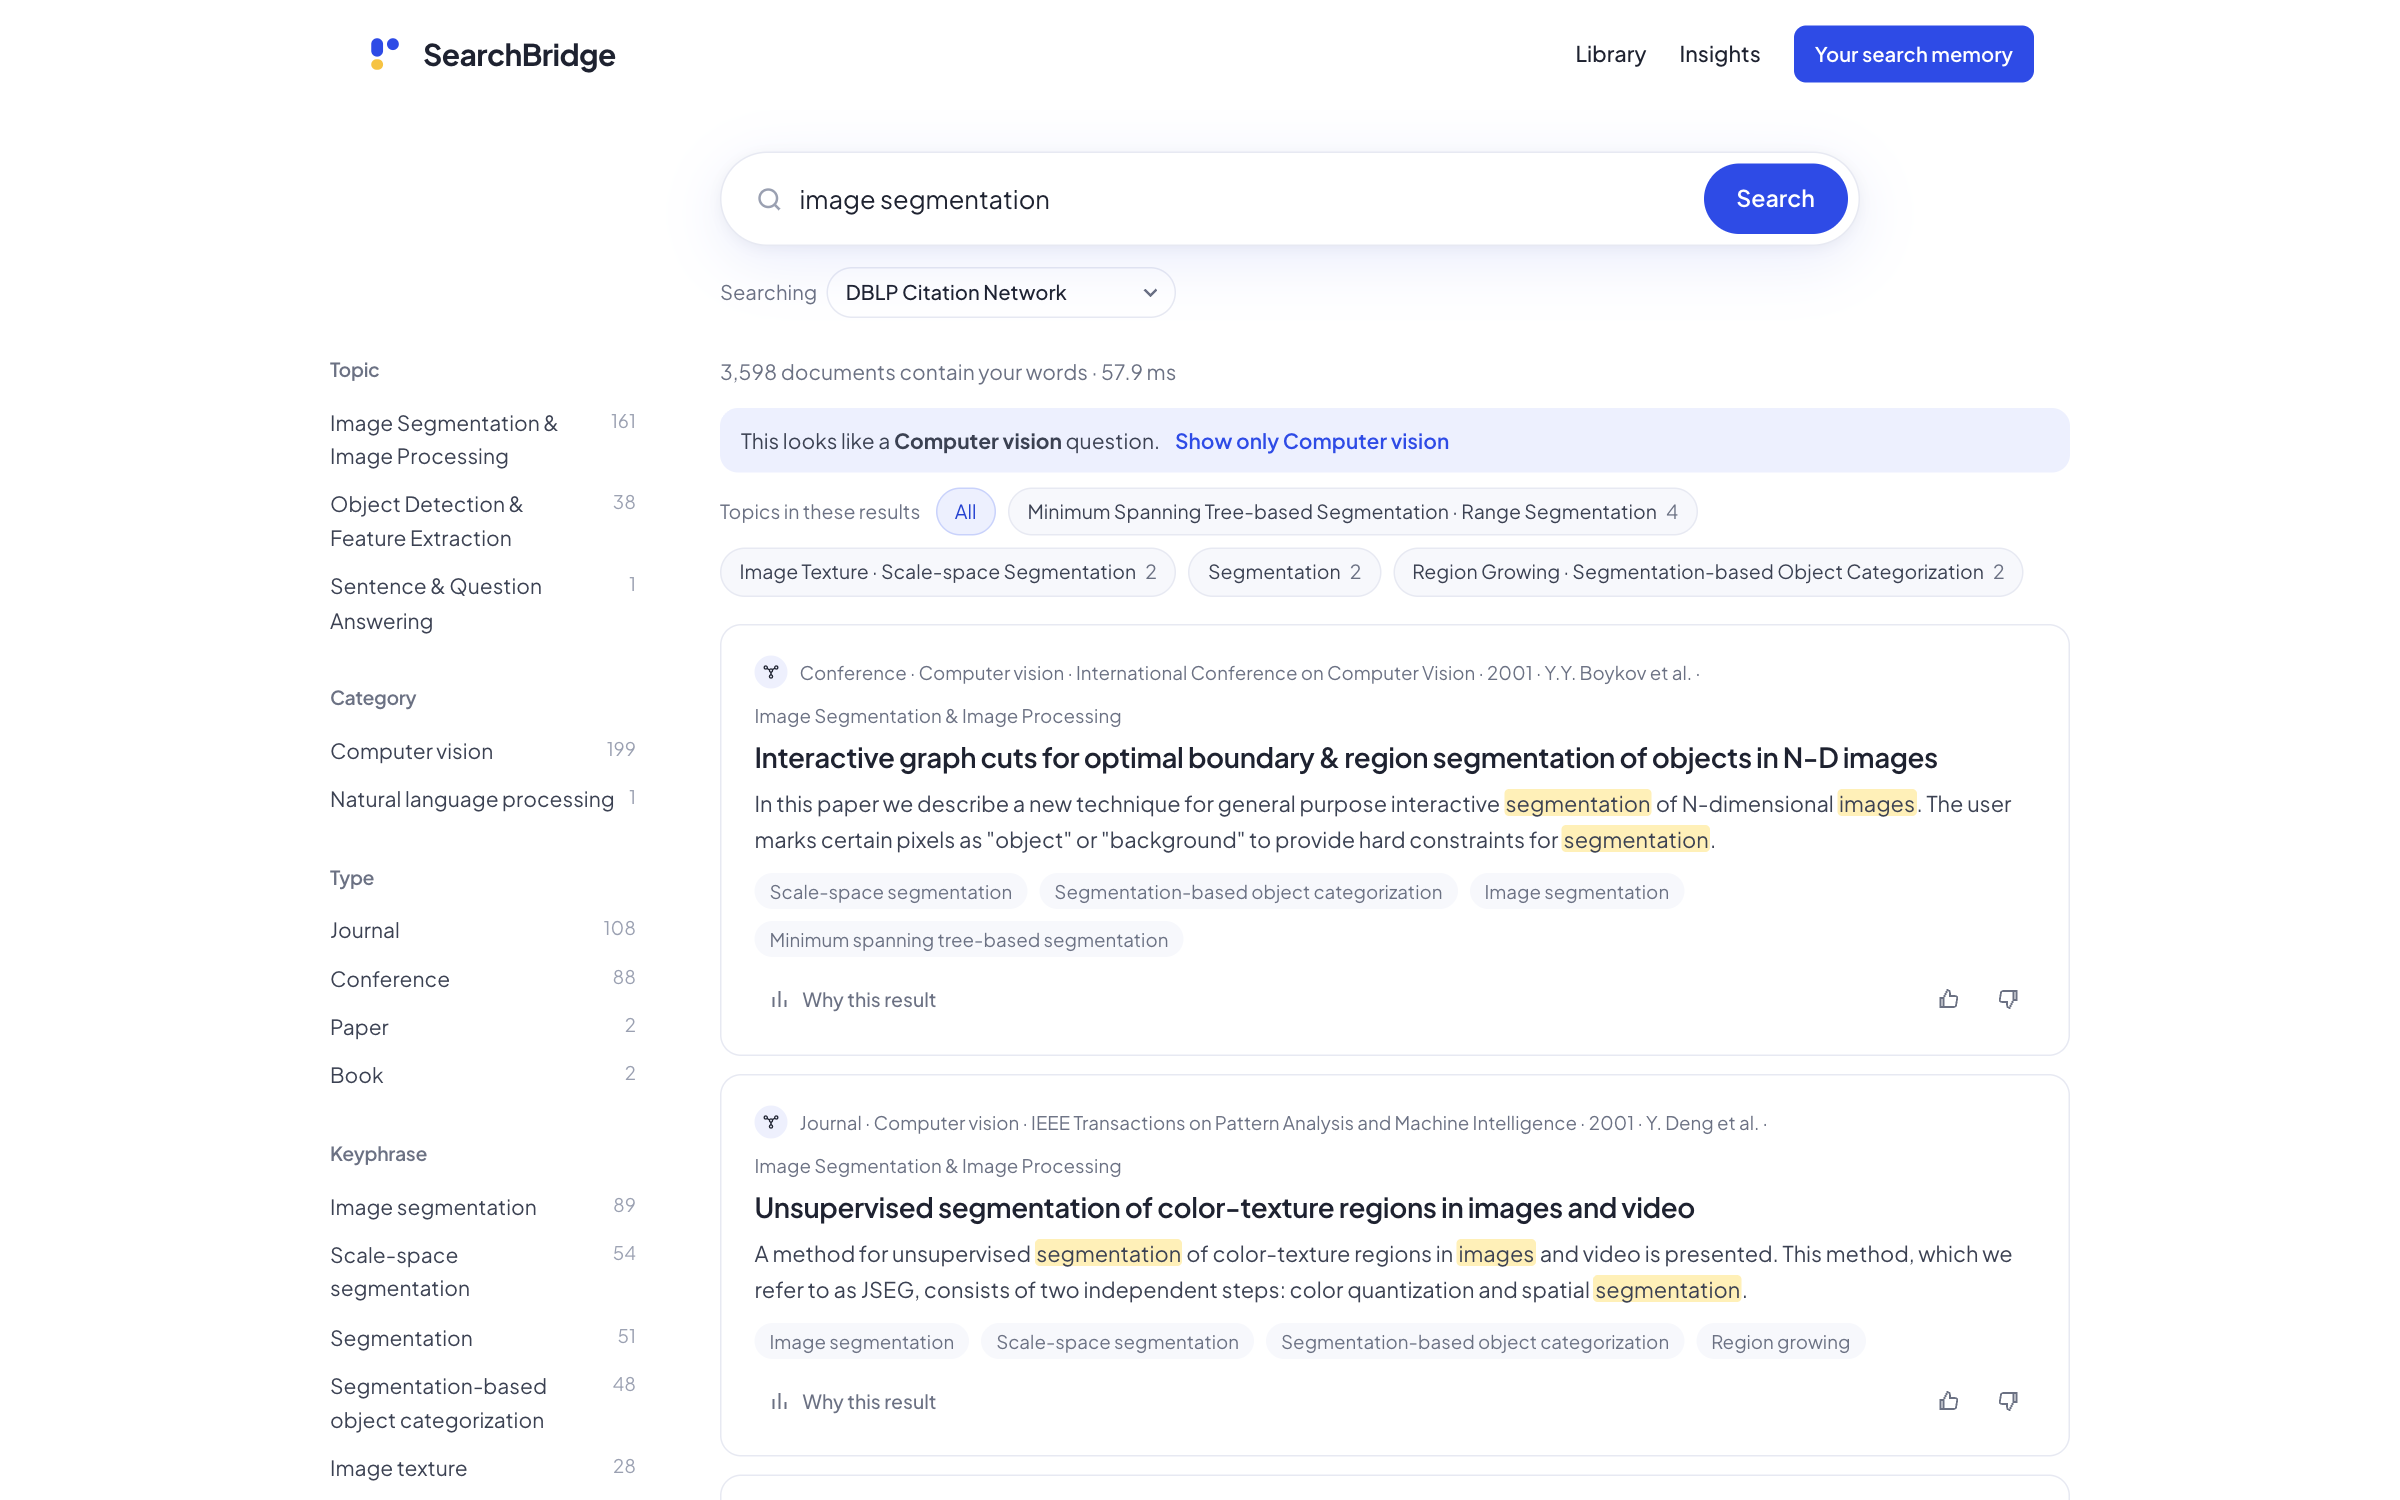
\includegraphics[width=0.92\textwidth]{02-search-results.png}
\caption{The SearchBridge search page for ``image segmentation'' on the DBLP collection: facets (left), the predicted field of the query, result-cluster chips and ranked results with highlighted snippets.}
\label{fig:ui}
\end{figure*}

%=====================================================================
\section{Literature Review}
\textbf{Probabilistic ranking.} Robertson and Zaragoza~\cite{robertson2009} derive BM25 from the probabilistic relevance framework, combining term frequency saturation ($k_1$) with document-length normalisation ($b$). It remains a strong baseline, and we use it as ours. Metzler and Croft~\cite{metzler2005} model term dependence with a Markov random field, rewarding query words that appear close together; we implement their sequential dependence model.

\textbf{Relevance feedback and query expansion.} Rocchio~\cite{rocchio1971} moves the query vector toward documents marked relevant and away from non-relevant ones. Lavrenko and Croft~\cite{lavrenko2001} estimate a relevance model from the top-ranked documents, and its interpolation with the original query (RM3)~\cite{abduljaleel2004} is the standard lexical pseudo-relevance feedback (PRF) method. Li et al.~\cite{li2023} show that PRF also helps dense retrievers when the query embedding is moved toward the feedback documents, but that the feedback set comes from the same dense retriever, so it inherits its errors.

\textbf{Semantic and hybrid retrieval.} Latent semantic analysis~\cite{deerwester1990} and Sentence-BERT~\cite{reimers2019} map queries and documents to vectors so that different words with the same meaning match. Cormack et al.~\cite{cormack2009} show that reciprocal-rank fusion (RRF) of several rankings outperforms individual systems. Arabzadeh et al.~\cite{arabzadeh2021} use query performance prediction~\cite{shtok2012,zhou2007} to decide, per query, whether sparse or dense retrieval should be used.

\textbf{Link analysis and duplicates.} Brin and Page~\cite{brin1998} rank pages by the stationary distribution of a random surfer with teleportation; Leskovec et al.~\cite{leskovec2020} explain why dead ends and spider traps require the full version; Haveliwala~\cite{haveliwala2002} makes the teleport topic-sensitive. Kleinberg's HITS~\cite{kleinberg1999} computes query-dependent hub and authority scores. Broder~\cite{broder1997} estimates document resemblance with MinHash, which locality-sensitive hashing makes scalable~\cite{leskovec2020}.

\textbf{Implicit feedback.} Fox et al.~\cite{fox2005} show that dwell time and return behaviour indicate satisfaction, and Agichtein et al.~\cite{agichtein2006} improve web ranking with such behaviour signals.

\subsection{Novelty of Our Approach}
\begin{enumerate}
\item \textbf{Bridged feedback.} RM3~\cite{abduljaleel2004} expands only the lexical query and dense PRF~\cite{li2023} only the embedding, each from its own retriever's results. Bridge-PRF takes one feedback set from the \emph{fused} ranking and applies it to \emph{both} representations, then fuses again. It outperforms RRF~\cite{cormack2009}, RM3 and dense PRF on Cranfield (Section~\ref{sec:compare}).
\item \textbf{Collection-relative gating.} Instead of fixed similarity thresholds, SearchBridge uses the previous query as context only when it is over-represented among the current query's candidates, and uses link authority only when the link graph covers enough of the collection. Both tests are relative to the collection, so they work for any encoder.
\item \textbf{Explainable, bounded personalization} built on implicit-feedback findings~\cite{fox2005,agichtein2006}, evaluated with an explicit harm check.
\item \textbf{One system for the whole syllabus}, where every ranking can be explained and every component is measured on its own, including ground-truth testing of the deployed system.
\end{enumerate}

%=====================================================================
\section{Objective}
The objectives of the project were to:
\begin{enumerate}
\item implement every syllabus topic (Boolean and ranked retrieval, indexing, crawling, PageRank and HITS, classification, clustering, relevance feedback, BM25) as part of one working search engine;
\item add the advanced features of semantic and hybrid search, query expansion and reformulation, context, suggestions, duplicate detection, personalization and explanations;
\item design a hybrid feedback method that beats BM25 and published fusion and feedback methods on a standard test collection;
\item evaluate every component with standard metrics (precision, recall, F1, accuracy, MAP, nDCG) on suitable datasets, with significance tests and cross-validation; and
\item make the system explain its rankings and verify its answers against ground truth.
\end{enumerate}

%=====================================================================
\section{Proposed Model}
Fig.~\ref{fig:arch} shows the proposed model. Documents enter from a web crawler, from user uploads (PDF, HTML, Markdown, JSON) or from a dataset. The same analyzer is applied to documents and to queries. Indexing builds four structures: a positional inverted index, a $k$-gram index over the vocabulary, document embeddings and the link graph. At query time one of eleven retrieval modes scores the documents; the default, Smart mode, runs Bridge-PRF and then adds bounded link, context and personal evidence before the results are de-duplicated, explained and returned. Classifiers, clustering, duplicate detection and a concept graph are computed once per collection; the engine is cached, so a restart takes seconds. A FastAPI service serves a JavaScript front end.

\begin{figure}[t]
\centering
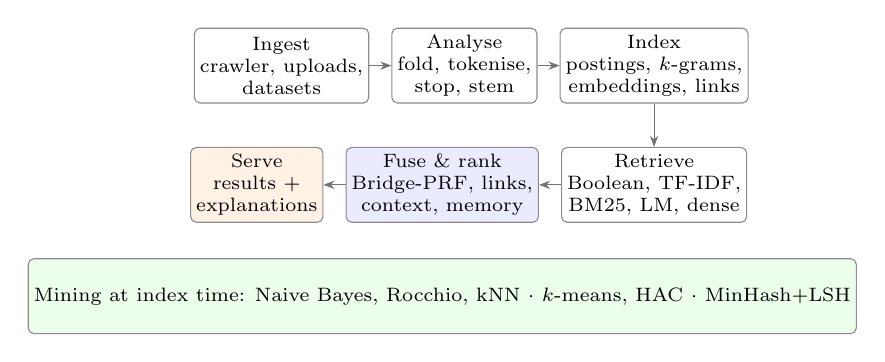
\begin{tikzpicture}[
  box/.style={draw=black!45, rounded corners=2pt, fill=#1, align=center, font=\scriptsize, minimum width=1.5cm, minimum height=0.95cm, inner sep=2pt},
  box/.default=white, arr/.style={-{Stealth[length=4pt]}, black!55}, node distance=0.28cm]
\node[box] (in) {Ingest\\crawler, uploads,\\datasets};
\node[box, right=of in] (an) {Analyse\\fold, tokenise,\\stop, stem};
\node[box, right=of an] (ix) {Index\\postings, $k$-grams,\\embeddings, links};
\node[box, below=0.55cm of ix] (rt) {Retrieve\\Boolean, TF-IDF,\\BM25, LM, dense};
\node[box=blue!8, left=of rt] (fu) {Fuse \& rank\\Bridge-PRF, links,\\context, memory};
\node[box=orange!10, left=of fu] (out) {Serve\\results +\\explanations};
\node[box=green!8, below=0.45cm of fu, minimum width=6.2cm] (mn) {Mining at index time: Naive Bayes, Rocchio, kNN $\cdot$ $k$-means, HAC $\cdot$ MinHash+LSH};
\draw[arr] (in) -- (an); \draw[arr] (an) -- (ix); \draw[arr] (ix) -- (rt); \draw[arr] (rt) -- (fu); \draw[arr] (fu) -- (out);
\end{tikzpicture}
\caption{Proposed model: the SearchBridge pipeline.}
\label{fig:arch}
\end{figure}

Fig.~\ref{fig:bridge} details Bridge-PRF, the core of Smart mode. A first pass fuses BM25 and semantic scores; the top $k$ fused documents form one shared feedback set; that set expands the lexical query with RM3 and moves the query embedding toward the feedback centroid; the two second-pass scores are fused again.

\begin{figure}[t]
\centering
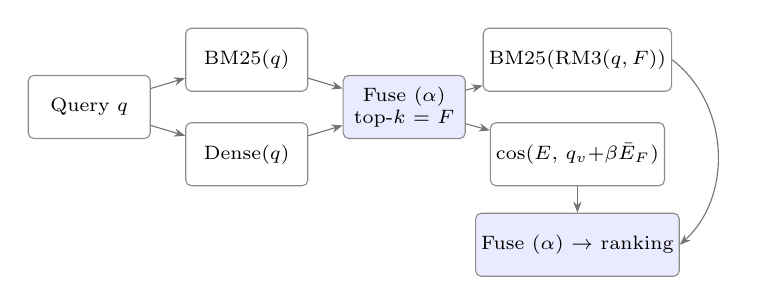
\begin{tikzpicture}[
  b/.style={draw=black!45, rounded corners=2pt, fill=#1, align=center, font=\scriptsize, minimum width=1.55cm, minimum height=0.8cm, inner sep=2pt},
  b/.default=white, arr/.style={-{Stealth[length=4pt]}, black!55}]
\node[b] (q) at (0,0) {Query $q$};
\node[b] (l0) at (2.0,0.6) {BM25$(q)$};
\node[b] (d0) at (2.0,-0.6) {Dense$(q)$};
\node[b=blue!8] (h0) at (4.0,0) {Fuse ($\alpha$)\\top-$k$ = $F$};
\node[b] (l1) at (6.2,0.6) {BM25(RM3$(q,F)$)};
\node[b] (d1) at (6.2,-0.6) {cos$(E,\,q_v{+}\beta\bar E_F)$};
\node[b=blue!8] (h1) at (6.2,-1.75) {Fuse ($\alpha$) $\rightarrow$ ranking};
\draw[arr] (q) -- (l0); \draw[arr] (q) -- (d0); \draw[arr] (l0) -- (h0); \draw[arr] (d0) -- (h0);
\draw[arr] (h0) -- (l1); \draw[arr] (h0) -- (d1);
\draw[arr] (l1.east) to[bend left=50] (h1.east); \draw[arr] (d1) -- (h1);
\end{tikzpicture}
\caption{Bridge-PRF: one feedback set from the fused first pass is fed back into both the lexical and the semantic retriever.}
\label{fig:bridge}
\end{figure}

\begin{table*}[t]
\caption{Syllabus topics and advanced features, how SearchBridge implements them, and the evidence that they work}
\label{tab:syllabus}
\centering\footnotesize
\begin{tabular}{@{}llp{6.0cm}p{5.3cm}@{}}
\toprule
& Topic & Implementation & Evidence \\
\midrule
\multirow{7}{*}{A} & 1. Boolean retrieval & AND/OR/NOT parser, phrases, $\sim k$ proximity, \texttt{*} and \texttt{?} wildcards & $|A\cup B|=|A|+|B|-|A\cap B|$ holds exactly \\
& 2. Text pre-processing & Unicode folding, SMART stop list, Porter stemmer & BM25 MAP 0.279 $\rightarrow$ 0.317 (Table~\ref{tab:prep}) \\
& 3. Ranked retrieval & Vector space model, \texttt{lnc.ltc}, cosine & Equals a hand calculation to 6 decimals \\
& 4. Scoring and result assembly & Fusion, filters, facets, snippets, de-duplication, paging & 60--140\,ms per query on 21,000 papers \\
& 5. Web crawler & BFS frontier, robots.txt, crawl delay, MinHash filter & 200 pages, 2,428 internal links \\
& 6. Evaluation & Precision, recall, F1, MAP, nDCG, BPref, randomisation test & 225 judged queries, 5-fold CV \\
& 7. Dictionary and inverted index & SPIMI, positional postings, $k$-gram index, VB/$\gamma$/$\delta$ codes & Postings 336\,KB $\rightarrow$ 81\,KB (Table~\ref{tab:prep}) \\
\midrule
\multirow{4}{*}{B} & 8--10. PageRank V1--V3 & Simplified, with teleportation, with dead-end handling & Rank kept 1.6\%, 45.9\%, 100\%; V3 equals networkx to $4\times10^{-9}$ \\
& 11. HITS & Hubs/authorities on the query's base set & Classic segmentation papers as authorities \\
\midrule
\multirow{4}{*}{C} & 12. Naive Bayes & Multinomial, Laplace smoothing, log space & F1 0.895 DBLP, 0.968 BBC (Table~\ref{tab:clf}) \\
& 13. Vector space classifier & Rocchio centroids and $k$NN ($k=5$) & F1 0.884 / 0.874 DBLP \\
& 14. Flat clustering & Spherical $k$-means with $k$-means++ & Purity 0.79 (Cranfield), 0.91 (BBC) \\
& 15. Hierarchical clustering & Single/complete/average-link HAC, dendrogram & Purity 0.65 complete link (Table~\ref{tab:clu}) \\
\midrule
\multirow{2}{*}{D} & 16. Relevance feedback & Rocchio (explicit), RM3 and vector PRF (pseudo) & Residual MAP 0.133 $\rightarrow$ 0.229 \\
& 17. BM25 & Okapi BM25 with per-term explanation & MAP 0.317 \\
\midrule
\multirow{10}{*}{Adv.} & Semantic search & Sentence-BERT, LSA fallback & MAP 0.359 vs.\ 0.317 for BM25 \\
& Hybrid retrieval & Min--max fusion, RRF, Bridge-PRF & MAP 0.386 \\
& Query expansion & RM3 terms, concept-graph related terms & Better than BM25 on 171 of 225 queries \\
& Query reformulation & Typo correction, Boolean repair & 0 wrong rewrites (previously 27) \\
& Context-aware retrieval & Earlier query blended in when related & In-field results 14 $\rightarrow$ 19 of 40 \\
& Query suggestions & Completions, titles, related topics, history & $O(\log V)$ prefix lookup \\
& Learning-to-rank & Learned fusion weight (QAHR) & \textcolor{orange!80!black}{Partial}: $r=0.08$ with oracle weight \\
& Near-duplicate detection & MinHash + LSH, Jaccard $\geq 0.8$ & BBC: 157 pairs, no false alarms \\
& Personalized retrieval & Time-decayed search memory, bounded boost & MAP 0.361 $\rightarrow$ 0.376, no harm when unrelated \\
& Explainable ranking & Score breakdown, term scores, missing words & On every result (Fig.~\ref{fig:why}) \\
\bottomrule
\end{tabular}
\end{table*}

%=====================================================================
\section{Methodology}
\subsection{Pre-processing and Indexing}
The analyzer applies NFKD Unicode folding (so ``na\"ive'' matches ``naive''), lower-casing, tokenisation with hyphen splitting, removal of a SMART-style stop list and one-letter tokens, and the Porter stemmer~\cite{porter1980}. For example, ``The Na\"ive Bayes classifiers were filtering e-mails in real-time systems'' becomes \texttt{naiv bay classifi filter mail real time system}.

The inverted index is built with single-pass in-memory indexing (SPIMI) and a $k$-way merge of sorted blocks~\cite{manning2008}. Postings store positions, which supports phrase and proximity queries. An auxiliary in-memory index supports dynamic additions, and deletions use an invalidation set. A bigram $k$-gram index over surface words serves wildcard queries and spelling correction. Postings are compressed by gap encoding with variable-byte, Elias $\gamma$ or $\delta$ codes, and the dictionary by front coding.

\subsection{Boolean Retrieval}
A recursive-descent parser with precedence NOT $>$ AND $>$ OR supports parentheses, implicit AND, quoted phrases, proximity (\texttt{"a b"$\sim$k}) and wildcards (\texttt{*} for any run of letters, \texttt{?} for one letter) expanded through the $k$-gram index. Conjunctions are evaluated shortest postings list first. Operands that contain no indexable term, such as stop words, are ignored rather than emptying the result.

\subsection{Ranked Retrieval}
All ranked models accumulate scores term-at-a-time over postings. The vector space model uses SMART \texttt{lnc.ltc} weighting: documents use $1+\log tf$ and queries $(1+\log tf)\cdot\log(N/df)$, both cosine-normalised~\cite{salton1988}. BM25~\cite{robertson2009} uses $k_1=1.2$, $b=0.75$:
\begin{equation}
\mathrm{BM25}(q,d)=\sum_{t\in q}\mathrm{idf}(t)\,\frac{tf_{t,d}\,(k_1+1)}{tf_{t,d}+k_1\left(1-b+b\frac{|d|}{\mathrm{avgdl}}\right)},
\end{equation}
with $\mathrm{idf}(t)=\ln\!\big(1+\frac{N-df_t+0.5}{df_t+0.5}\big)$. We also implement query likelihood with Dirichlet ($\mu=300$) and Jelinek--Mercer smoothing~\cite{zhai2004} and the sequential dependence model~\cite{metzler2005}. Semantic retrieval scores $\cos(E(q),E(d))$ with Sentence-BERT embeddings (all-MiniLM-L6-v2, 384 dimensions)~\cite{reimers2019}, or LSA (TF-IDF then a 200-dimensional truncated SVD)~\cite{deerwester1990} when the model is unavailable.

\subsection{Relevance Feedback and Bridge-PRF}
Explicit feedback uses Rocchio's formula~\cite{rocchio1971}
\begin{equation}
\vec q\,' = \alpha\,\vec q + \beta\,\frac{1}{|R|}\sum_{d\in R}\vec d - \gamma\,\frac{1}{|N\!R|}\sum_{d\in N\!R}\vec d,
\end{equation}
with $\alpha=1$, $\beta=0.75$, $\gamma=0.15$, keeping the 30 strongest positive terms. Bridge-PRF (Fig.~\ref{fig:bridge}) computes the first-pass hybrid score
\begin{equation}
H_0(d)=\alpha\,\widehat{L}_0(d)+(1-\alpha)\,\widehat{D}_0(d),
\end{equation}
where $\widehat{\cdot}$ denotes min--max normalisation of the BM25 and dense scores. The top $k$ documents $F$ of $H_0$ give (i) an RM3 query $\lambda\,P(w|q)+(1-\lambda)\,P(w|F)$ with $\lambda=0.6$ and 10 expansion terms~\cite{abduljaleel2004}, scored with BM25, and (ii) a dense query $q_v+\beta\,\overline{E_F}$ with $\beta=0.8$. The two second-pass scores are fused with the same $\alpha$. $k$ and $\alpha$ are chosen by cross-validation.

\subsection{Scoring, Context and Result Assembly}
Smart mode normalises the Bridge-PRF score to $[0,1]$ over the top 200 candidates and adds bounded terms: PageRank and HITS authority (at most 0.05 each), a context term and the user's search memory. Link terms are used only when at least 20\% of documents have links. The previous query is used as context only if the share of the top 200 candidates that fall in the 2\% of the collection most similar to it is at least three times the chance rate; the candidates are then re-scored against the normalised sum of both query embeddings and mixed in with weight 0.5. Field filters, facets, near-duplicate folding, query-biased snippets, pagination and MMR diversification~\cite{carbonell1998} complete the result page.

\subsection{Web Crawler}
The crawler keeps a breadth-first, normalised URL frontier with depth and page limits; obeys robots.txt and Crawl-delay; waits at least one second between requests to a host; restricts itself to allowed domains and path prefixes; skips exact duplicates by SHA-1 and near duplicates by MinHash; extracts the main content of a page while dropping navigation, sidebars and footers; and keeps only links between crawled pages.

\subsection{PageRank and HITS}
Following~\cite{leskovec2020}, three PageRank versions are kept separate. With $M$ the column-stochastic link matrix, $D$ the dead ends and $\beta=0.85$:
\begin{align}
\text{V1:}\quad & r \leftarrow M r,\\
\text{V2:}\quad & r \leftarrow \beta M r + (1-\beta)/N,\\
\text{V3:}\quad & r \leftarrow \beta\big(M r + \textstyle\sum_{i\in D} r_i\, v\big) + (1-\beta)\,v,
\end{align}
where $v$ is uniform or topic-specific~\cite{haveliwala2002}. HITS~\cite{kleinberg1999} takes the top 30 results as the root set, adds every paper they cite or are cited by, and iterates $a=A^{\top}h$, $h=Aa$ with normalisation.

\subsection{Classification and Clustering}
Multinomial Naive Bayes assigns $\hat c=\arg\max_c\big[\log P(c)+\sum_{t\in d}\log\frac{T_{ct}+1}{\sum_{t'}T_{ct'}+|V|}\big]$ (Laplace smoothing). Rocchio classifies by the nearest TF-IDF class centroid, and $k$NN ($k=5$) by cosine-weighted votes~\cite{manning2008}. A document without a category gets one only when Naive Bayes and Rocchio agree with probability at least 0.9; the classifiers also predict the field of each query. Spherical $k$-means with $k$-means++ seeding~\cite{arthur2007} groups each collection into $k=\mathrm{round}(\sqrt{N/10})$ topics (between 2 and 16); hierarchical agglomerative clustering (single, complete or average link, cosine distance) relates them in a dendrogram. Each cluster is named by the keyphrases whose share inside it most exceeds their share elsewhere.

\subsection{Near-Duplicate Detection}
Documents become sets of 4-word shingles. 64 MinHash values~\cite{broder1997} are split into $b=16$ LSH bands of $r=4$ rows, so a pair with Jaccard similarity $s$ is compared with probability $1-(1-s^r)^b$. Candidates are verified with the exact Jaccard similarity ($\geq 0.8$) and folded into one result.

\subsection{Query Reformulation, Suggestions, Personalization and Explanations}
Spelling correction finds candidates by $k$-gram overlap and ranks them by Damerau--Levenshtein distance and frequency; it corrects only likely typos and always offers the original spelling. Suggestions combine phrase completions checked against the positional index, matching titles, related topics from a concept graph, the user's history and popular queries shown only after several distinct users~\cite{sweeney2002}. Search memory~\cite{fox2005,agichtein2006} turns interactions into bounded evidence (opening $+0.25$, reading $\geq 30$\,s $+0.75$, quick return $-0.2$, explicit feedback $\pm1.5$) with a 21-day half-life and $\tanh$ saturation; its score is added with weight 0.5, gated by relevance. The ``Why this result'' panel (Fig.~\ref{fig:why}) shows the score components, each query word's BM25 contribution, the exact-word versus semantic split, missing query words and history reasons.

\begin{figure}[t]
\centering
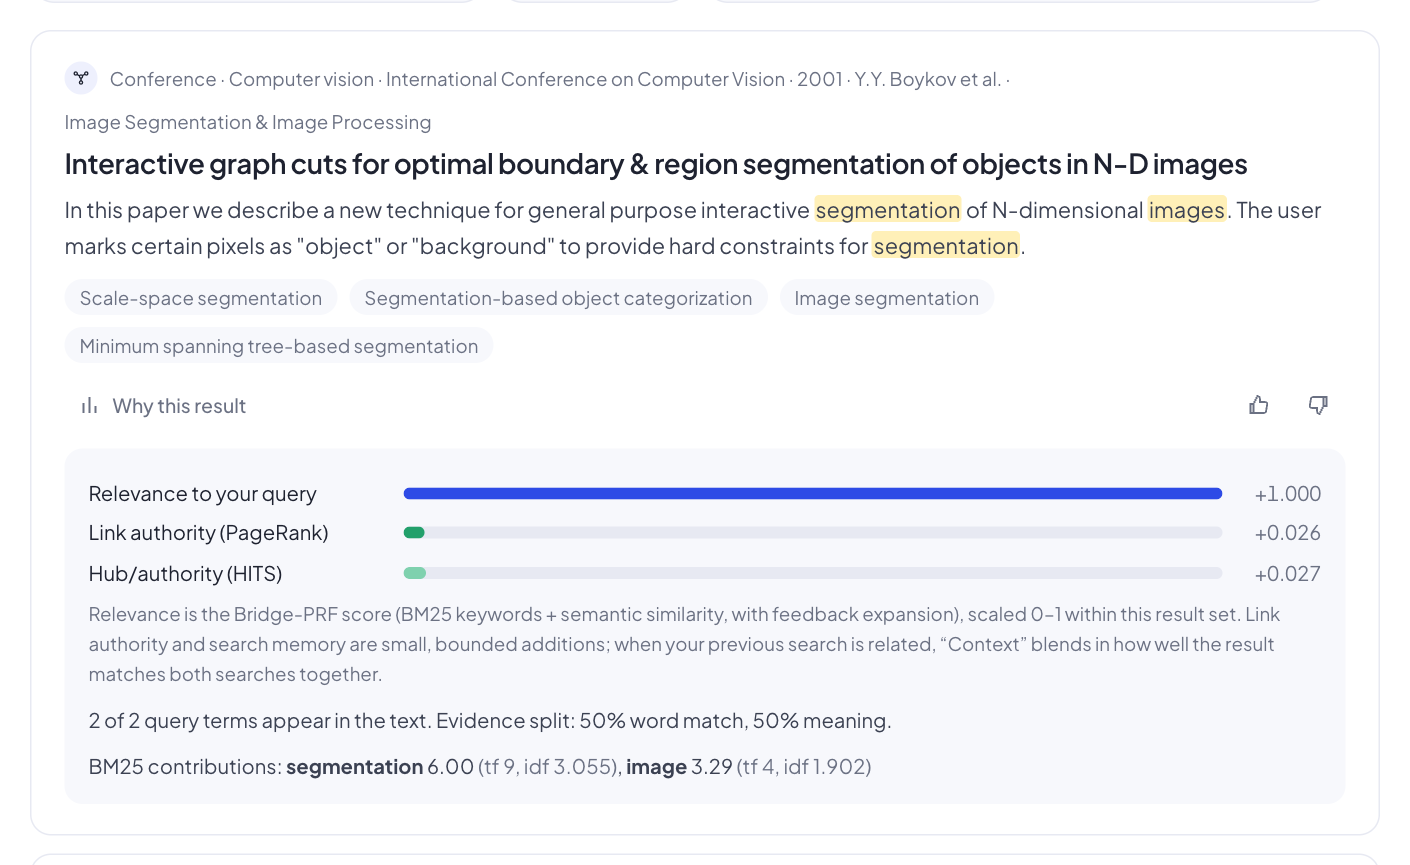
\includegraphics[width=\columnwidth]{c-why.png}
\caption{The ``Why this result'' panel: score components, term-level BM25 evidence and the word-versus-meaning split.}
\label{fig:why}
\end{figure}

%=====================================================================
\section{Experimentation and Results}
\subsection{Datasets}
Table~\ref{tab:collections} lists the six collections. Cranfield~\cite{cleverdon1967} has 225 queries with human relevance judgements and is used for ranking quality. From the 12\,GB DBLP-Citation-network V12 dump~\cite{tang2008} (4,894,081 papers) we kept every paper from 2000 onwards with a title and abstract, labelled it with the highest-weighted of six computer-science fields of study, and kept the 3,500 papers per field most cited by the other candidates; abstracts were rebuilt from DBLP's inverted-index encoding and only citations inside the sample were kept, so 98.6\% of the papers have a citation link. BBC News~\cite{greene2006} has five topic labels and contains real duplicate articles.

\begin{table}[t]
\caption{Datasets}
\label{tab:collections}
\centering\footnotesize
\setlength{\tabcolsep}{3pt}
\begin{tabular}{@{}lrll@{}}
\toprule
Collection & Docs & Links & Labels / judgements \\
\midrule
DBLP Citation Network & 21,000 & 165,793 & 6 CS fields \\
BBC News & 2,225 & -- & 5 topics \\
Cranfield 1400 & 1,400 & -- & 225 judged queries \\
Classic CS Papers & 2,243 & 40 & 4 fields (243 papers) \\
Web pages (own crawl) & 200 & 2,428 & -- \\
My Library & user files & -- & -- \\
\bottomrule
\end{tabular}
\end{table}

\subsection{Evaluation Metrics and Protocol}
For a query with relevant set $R$ and top-$k$ results $A_k$, precision is $P@k=|R\cap A_k|/k$, recall $R@k=|R\cap A_k|/|R|$ and $F_1@k=2\,P@k\,R@k/(P@k+R@k)$. Average precision averages $P@k$ over the ranks of relevant documents, and MAP averages it over queries. We also report nDCG@10~\cite{jarvelin2002} and BPref~\cite{buckley2004}. Classifiers are measured by accuracy and macro-averaged precision, recall and F1 on a stratified 80/20 split, and clusters by purity and normalised mutual information (NMI). Every tuned ranking system is evaluated with 5-fold cross-validation over queries, and differences in per-query average precision are tested with a two-sided paired randomisation test (10,000 permutations)~\cite{smucker2007}.

\subsection{Retrieval Effectiveness}
Table~\ref{tab:main} reports the retrieval models on Cranfield, and Table~\ref{tab:prf} the full system as deployed, with precision, recall and F1 at 10. Fig.~\ref{fig:prc} shows the precision--recall curves. Lexical models reach MAP 0.30--0.32, LSA alone 0.359, and feedback improves every model. Bridge-PRF is best at MAP 0.386 (+22\% over BM25) and P@10 0.294, better than BM25 on 171 of 225 queries (Fig.~\ref{fig:delta}).

\begin{table}[t]
\caption{Retrieval effectiveness on Cranfield (depth 1,000). $\dagger$: significantly different from BM25 ($p<0.05$)}
\label{tab:main}
\centering\footnotesize
\setlength{\tabcolsep}{4pt}
\begin{tabular}{@{}lcccc@{}}
\toprule
System & MAP & P@10 & R@100 & nDCG@10 \\
\midrule
TF-IDF (\texttt{lnc.ltc}) & 0.308 & 0.235 & 0.760 & 0.386 \\
BM25 & 0.317 & 0.238 & 0.751 & 0.391 \\
QL-LM, Dirichlet & 0.302$^\dagger$ & 0.230 & 0.738 & 0.381 \\
SDM / MRF & 0.306$^\dagger$ & 0.234 & 0.743 & 0.388 \\
Semantic (LSA) & 0.359$^\dagger$ & 0.268 & 0.804 & 0.435 \\
Hybrid, linear (CV) & 0.359$^\dagger$ & 0.272 & 0.798 & 0.437 \\
QAHR, adaptive (CV) & 0.357$^\dagger$ & 0.272 & 0.795 & 0.435 \\
\textbf{Bridge-PRF (CV)} & \textbf{0.386}$^\dagger$ & \textbf{0.294} & \textbf{0.827} & \textbf{0.464} \\
\bottomrule
\end{tabular}
\end{table}

\begin{table}[t]
\caption{Deployed system on Cranfield: precision, recall and F1 at 10}
\label{tab:prf}
\centering\footnotesize
\begin{tabular}{@{}lcccc@{}}
\toprule
Mode & P@10 & R@10 & F1@10 & MAP \\
\midrule
Boolean (AND of query words) & 0.009 & 0.016 & 0.011 & 0.014 \\
TF-IDF & 0.232 & 0.400 & 0.265 & 0.299 \\
BM25 & 0.235 & 0.396 & 0.267 & 0.307 \\
Semantic (LSA) & 0.267 & 0.452 & 0.304 & 0.350 \\
Hybrid & 0.261 & 0.437 & 0.296 & 0.346 \\
\textbf{Smart (Bridge-PRF)} & \textbf{0.291} & \textbf{0.481} & \textbf{0.327} & \textbf{0.372} \\
\bottomrule
\end{tabular}
\end{table}

\begin{figure}[t]
\centering
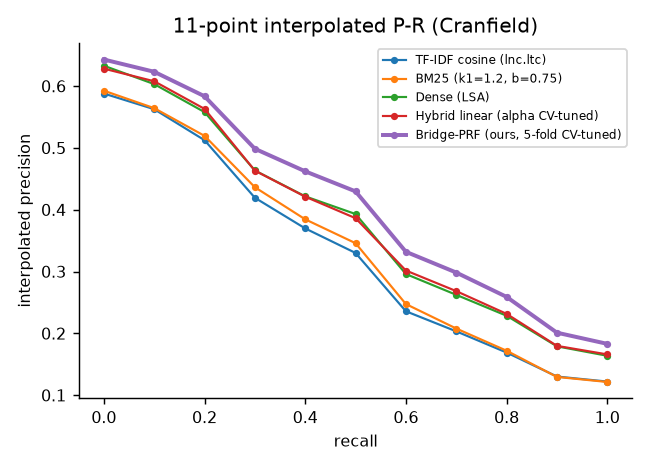
\includegraphics[width=0.92\columnwidth]{pr_curves.png}
\caption{Interpolated 11-point precision--recall curves on Cranfield.}
\label{fig:prc}
\end{figure}

\begin{figure}[t]
\centering
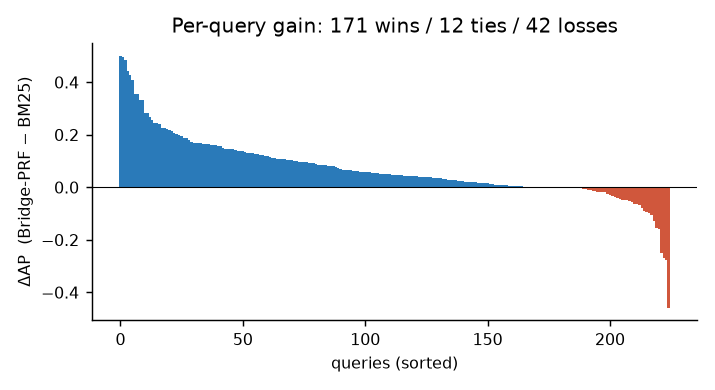
\includegraphics[width=\columnwidth]{per_query_delta.png}
\caption{Per-query difference in average precision, Bridge-PRF minus BM25, sorted: 171 queries improve, 12 tie and 42 get worse.}
\label{fig:delta}
\end{figure}

\subsection{Comparison with Existing Research}\label{sec:compare}
Table~\ref{tab:compare} compares Bridge-PRF with the methods proposed in four published papers, each re-implemented by us and run on the same Cranfield queries, judgements and index, so the comparison is like for like. Bridge-PRF outperforms RRF~\cite{cormack2009} by 10\%, RM3~\cite{abduljaleel2004} by 9\% and the per-query adaptive fusion in the spirit of Arabzadeh et al.~\cite{arabzadeh2021} by 8\% (paired randomisation test, $p<0.001$ in each case). Its advantage over dense PRF~\cite{li2023} (+2.3\%) is not statistically significant ($p=0.14$).

\begin{table}[t]
\caption{Bridge-PRF vs.\ re-implemented methods from published papers (Cranfield). $\ddagger$: Bridge-PRF significantly better ($p<0.001$)}
\label{tab:compare}
\centering\footnotesize
\setlength{\tabcolsep}{4pt}
\begin{tabular}{@{}llcc@{}}
\toprule
Method & Paper & MAP & P@10 \\
\midrule
BM25 & Robertson \& Zaragoza~\cite{robertson2009} & 0.317$^\ddagger$ & 0.238 \\
Reciprocal-rank fusion & Cormack et al.~\cite{cormack2009} & 0.350$^\ddagger$ & 0.263 \\
BM25 + RM3 & Abdul-Jaleel et al.~\cite{abduljaleel2004} & 0.354$^\ddagger$ & 0.268 \\
QPP-adaptive fusion & cf.\ Arabzadeh et al.~\cite{arabzadeh2021} & 0.357$^\ddagger$ & 0.272 \\
Dense + vector PRF & Li et al.~\cite{li2023} & 0.377 & 0.283 \\
\textbf{Bridge-PRF} & this work & \textbf{0.386} & \textbf{0.294} \\
\bottomrule
\end{tabular}
\end{table}

\subsection{Ablation and Negative Results}
Table~\ref{tab:abl} removes one part of Bridge-PRF at a time. Removing feedback entirely costs 0.018 MAP and removing the dense branch costs 0.013, while removing the lexical branch costs only 0.003. Replacing the shared hybrid feedback set by each retriever's own top documents gives 0.3784 against 0.3785: \emph{the gain comes from applying feedback to both representations, not from sharing the feedback set}. We report this honestly, as it narrows our novelty claim to the dual-sided use of hybrid feedback.

Two further ideas did not work. QAHR, our learned per-query fusion weight, correlates with the oracle weight at only $r=0.084$ and scores slightly below a single cross-validated weight (0.357 vs.\ 0.359), although an oracle per-query weight would reach 0.394. PageRank computed over a similarity graph lowered MAP on Cranfield from 0.379 to 0.373, so SearchBridge never synthesises links.

\begin{table}[t]
\caption{Bridge-PRF ablation on Cranfield ($k=5$, $\alpha=0.3$)}
\label{tab:abl}
\centering\footnotesize
\begin{tabular}{@{}lcc@{}}
\toprule
Variant & MAP & P@10 \\
\midrule
Full Bridge-PRF & 0.3785 & 0.292 \\
\quad without lexical RM3 branch & 0.3753 & 0.285 \\
\quad without dense vector-PRF branch & 0.3659 & 0.276 \\
\quad self feedback instead of shared & 0.3784 & 0.292 \\
\quad no feedback (hybrid fusion only) & 0.3602 & 0.272 \\
\bottomrule
\end{tabular}
\end{table}

\subsection{Pre-processing and Index}
Table~\ref{tab:prep} shows that stemming and stop-word removal together raise BM25 MAP from 0.279 to 0.317 while shrinking the vocabulary by 37\%, and that $\gamma$-coded gaps store postings in 24\% of the uncompressed size; front coding shrinks the dictionary by 61\%. Zipf's law holds with exponent 0.93 and Heaps' law with $M=24\,T^{0.45}$. Boolean retrieval satisfies set identities exactly: \textit{boundary} (470 documents) OR \textit{layer} (414) gives $470+414-371=513$, NOT \textit{boundary} gives $1{,}400-470=930$, and the phrase ``boundary layer'' matches 367 documents against 4 for the reversed phrase.

\begin{table}[t]
\caption{Text processing and index compression (Cranfield)}
\label{tab:prep}
\centering\footnotesize
\begin{tabular}{@{}lrr@{}}
\toprule
BM25 with & MAP & Vocabulary \\
\midrule
no stemming, stop words kept & 0.279 & 7,436 \\
no stemming, stop words removed & 0.295 & 7,319 \\
stemming, stop words kept & 0.303 & 4,786 \\
stemming, stop words removed & \textbf{0.317} & 4,676 \\
\midrule
Postings structure & Bytes & Ratio \\
\midrule
4-byte integers & 335,808 & 1.000 \\
gaps + variable-byte & 91,755 & 0.273 \\
gaps + Elias $\gamma$ & 81,097 & 0.241 \\
gaps + Elias $\delta$ & 80,928 & 0.241 \\
\bottomrule
\end{tabular}
\end{table}

\subsection{Link Analysis}
On the DBLP graph (165,793 citations, 2,375 dead ends), V1 retains only 1.6\% of the total rank after 100 iterations because rank leaks through dead ends; V2 fixes spider traps but retains 45.9\%; V3 keeps the total at 1 and converges in 110 iterations (Fig.~\ref{fig:pr}). V3 matches networkx to within $4\times10^{-9}$, and its top paper is Collins' head-driven statistical parsing paper. For ``image segmentation'', HITS builds a base set of 350 papers and 2,202 links; the top authorities are Felzenszwalb and Huttenlocher's graph-based segmentation, Normalized Cuts and GrabCut, and the hubs are surveys that cite them.

\begin{figure}[t]
\centering
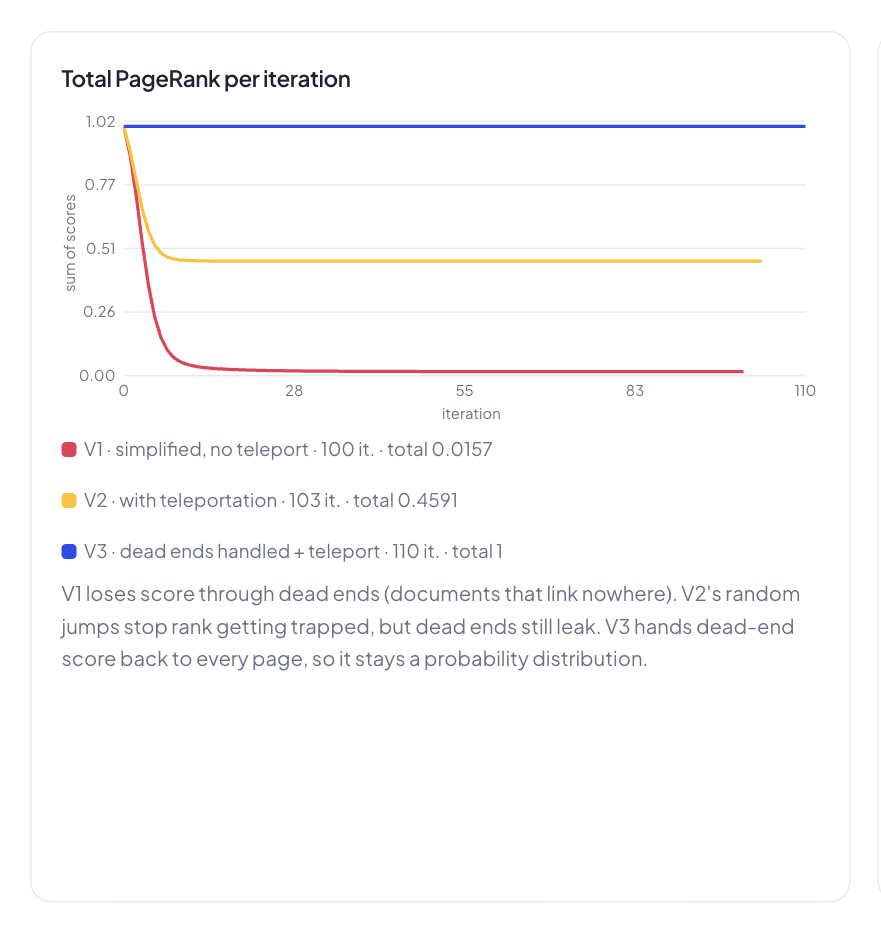
\includegraphics[width=0.78\columnwidth]{c-pagerank.png}
\caption{Total PageRank per iteration on the DBLP citation graph: V1 leaks rank through dead ends, V2 still leaks, V3 conserves it.}
\label{fig:pr}
\end{figure}

\subsection{Classification}
Table~\ref{tab:clf} reports held-out accuracy and macro-averaged precision, recall and F1. Naive Bayes is best on both datasets, and all three classifiers are far above the majority-class baseline. Our Naive Bayes agrees with scikit-learn's on every test document we compared. Used live, the classifiers label the field of 21 of 22 test queries correctly with none wrong.

\begin{table}[t]
\caption{Classification on held-out documents}
\label{tab:clf}
\centering\footnotesize
\setlength{\tabcolsep}{3.5pt}
\begin{tabular}{@{}llcccc@{}}
\toprule
Dataset & Classifier & Acc. & Prec. & Rec. & F1 \\
\midrule
\multirow{4}{*}{\shortstack[l]{DBLP\\6 fields\\4,200 test}} & Naive Bayes & \textbf{0.896} & \textbf{0.895} & \textbf{0.896} & \textbf{0.895} \\
& Rocchio & 0.885 & 0.884 & 0.885 & 0.884 \\
& $k$NN ($k=5$) & 0.875 & 0.874 & 0.875 & 0.874 \\
& Majority class & 0.167 & -- & -- & -- \\
\midrule
\multirow{4}{*}{\shortstack[l]{BBC\\5 topics\\444 test}} & Naive Bayes & \textbf{0.969} & \textbf{0.968} & \textbf{0.968} & \textbf{0.968} \\
& Rocchio & 0.962 & 0.960 & 0.961 & 0.960 \\
& $k$NN ($k=5$) & 0.957 & 0.956 & 0.957 & 0.956 \\
& Majority class & 0.230 & -- & -- & -- \\
\bottomrule
\end{tabular}
\end{table}

\subsection{Clustering}
Table~\ref{tab:clu} compares clustering methods on 179 Cranfield documents whose topic is known from the relevance judgements of eight queries with disjoint relevant sets. $k$-means is the most reliable; average-link HAC chains into one large cluster early. Without seeing labels, the automatic topics reach purity 0.913 (NMI 0.632) on BBC News and 0.836 (NMI 0.566) on DBLP (Fig.~\ref{fig:topics}).

\begin{table}[t]
\caption{Clustering 179 Cranfield documents into 8 known topics}
\label{tab:clu}
\centering\footnotesize
\begin{tabular}{@{}lcc@{}}
\toprule
Method & Purity & NMI \\
\midrule
$k$-means (spherical), LSA vectors & \textbf{0.788} & \textbf{0.715} \\
HAC, complete link, LSA vectors & 0.654 & 0.619 \\
HAC, average link, LSA vectors & 0.408 & 0.419 \\
$k$-means on TF-IDF vectors & 0.687 & 0.560 \\
Random assignment & 0.285 & 0.068 \\
\bottomrule
\end{tabular}
\end{table}

\begin{figure}[t]
\centering
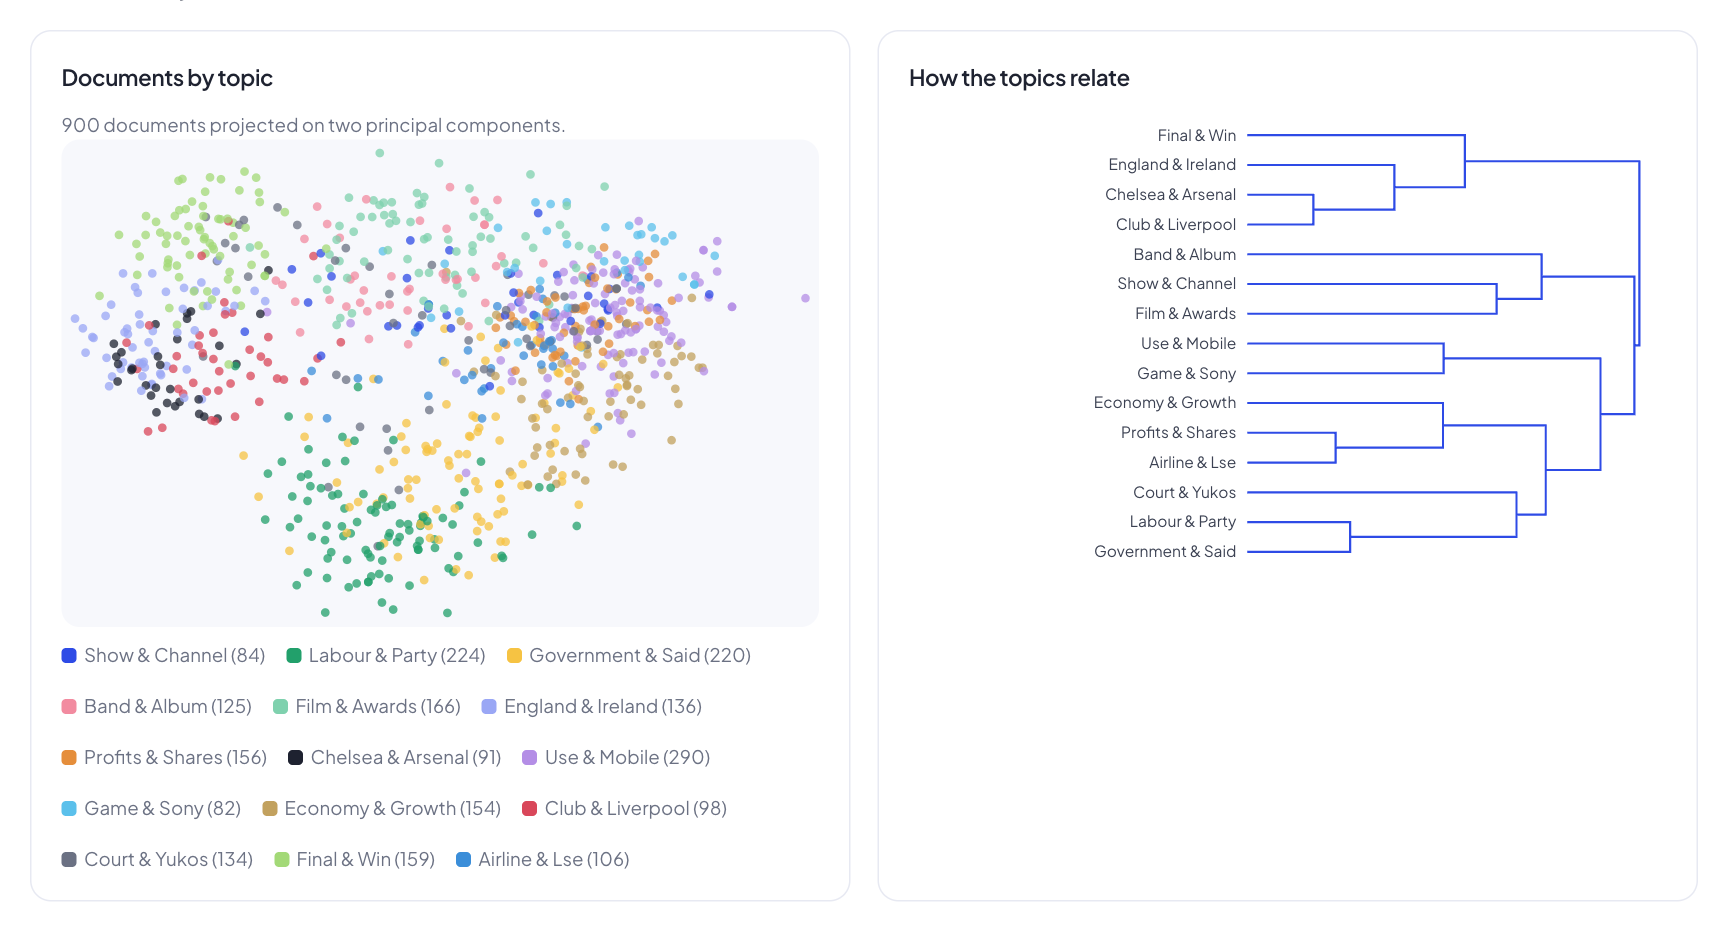
\includegraphics[width=\columnwidth]{c-topics.png}
\caption{BBC News topics: documents projected onto two principal components and coloured by $k$-means topic (left); average-link dendrogram of the topic centroids (right).}
\label{fig:topics}
\end{figure}

\subsection{Duplicates, Context and Personalization}
With 16 bands of 4 rows, a pair is compared with probability 12\% at Jaccard 0.3, 64\% at 0.5 and 99.98\% at 0.8. In BBC News this finds 157 pairs, 134 identical and 23 lightly edited copies of the same story, with no false alarms and no identical copy missed. Context-aware retrieval raised the number of top-10 results in the earlier query's field from 14 to 19 of 40 on eight ambiguous DBLP queries, and unrelated earlier queries were never used. Table~\ref{tab:pers} evaluates search memory with simulated users on Cranfield's real judgements: it helps related and repeated searches, does nothing on unrelated ones, and fades after 120 days.

\begin{table}[t]
\caption{Search memory with simulated users (Cranfield MAP, 2-fold CV)}
\label{tab:pers}
\centering\footnotesize
\begin{tabular}{@{}lccc@{}}
\toprule
Scenario & Without & With & $p$ \\
\midrule
Related later search & 0.361 & \textbf{0.376} & $<0.001$ \\
Same search again & 0.361 & \textbf{0.409} & $<0.001$ \\
Unseen documents only & 0.325 & 0.330 & $<0.001$ \\
Unrelated search (harm check) & 0.372 & 0.372 & 0.57 \\
Related, 120 days later & 0.361 & 0.361 & 0.45 \\
\bottomrule
\end{tabular}
\end{table}

\subsection{Testing the Deployed System}
Beyond 80 unit tests, we test the running system end to end with 88 HTTP checks whose expected answers come from ground truth: relevance judgements, category labels and set identities. This found eight real defects (Table~\ref{tab:bugs}), all fixed and covered by regression tests. Fixing them raised the deployed system's P@10 on Cranfield from 0.222 to 0.235 for BM25 and from 0.274 to 0.291 for Smart mode. The benchmark results in Table~\ref{tab:main} call the models directly and were not affected.

\begin{table}[t]
\caption{Defects found by ground-truth end-to-end testing}
\label{tab:bugs}
\centering\footnotesize
\setlength{\tabcolsep}{3pt}
\begin{tabular}{@{}>{\raggedright\arraybackslash}p{3.0cm}>{\raggedright\arraybackslash}p{2.5cm}>{\raggedright\arraybackslash}p{2.3cm}@{}}
\toprule
Defect & Before & After fix \\
\midrule
Parenthesis turned a query Boolean & 12/225 queries returned nothing & 0 \\
Stop word inside an AND & ``the AND boundary'' $\rightarrow$ 0 & 470 results \\
\texttt{?} wildcard & never matched & h?at $\rightarrow$ heat \\
Spelling rewrote real words & 27/225 queries & 0 \\
Link bonus on sparse graph & reordered top result & off below 20\% links \\
Gibberish query & 10 confident results & ``nothing matches'' \\
Context never changed ranking & 14/40 in field & 19/40 in field \\
Zipf exponent misfitted & 1.63 & 0.93 \\
\bottomrule
\end{tabular}
\end{table}

\subsection{Discussion}
Three lessons stand out. First, \emph{feedback matters more than fusion}: fusing BM25 and semantic scores alone (MAP 0.359) gains little over the semantic model, while feeding the fused results back into both retrievers reaches 0.386; the dense side benefits most, consistent with Li et al.~\cite{li2023}. Second, \emph{link analysis helps only on real, dense graphs}: on DBLP it identifies the classic papers, while synthetic or sparse graphs hurt. Third, classical classifiers remain strong on topical text, and Naive Bayes, the simplest, is the best. Finally, testing the deployed system against ground truth revealed defects that benchmark scripts, which bypass the user-facing pipeline, could not see.

%=====================================================================
\section{Conclusions and Limitations}
\subsection{Conclusions}
SearchBridge AI shows that the whole IR syllabus, from Boolean retrieval to PageRank, classification and clustering, can be combined into one usable, explainable search engine. Bridge-PRF improves MAP by 22\% over BM25 and outperforms re-implementations of RRF, RM3 and adaptive fusion; Naive Bayes reaches F1 0.895 on DBLP and 0.968 on BBC News; and every result can be explained to the user. Measuring every component on its own, including the deployed system, is what turned a collection of algorithms into a trustworthy system.

\subsection{Limitations}
(1) Learning-to-rank is only partial: the learned fusion weight is weak, and a pairwise reranker over the features we already compute is the natural next step. (2) All ranking results rest on one small, old judged collection; BEIR collections such as SciFact and NFCorpus would test generality. (3) Bridge-PRF's advantage over dense PRF alone is not significant, and the ablation shows that sharing the feedback set adds nothing by itself. (4) Search memory is evaluated with simulated users only. (5) The stored web crawl predates the content extractor and should be re-crawled. (6) Explanations are word-level only for the lexical part of the score. (7) Exact vector search suits collections up to about $10^5$ documents; larger ones need an approximate nearest-neighbour index.

%=====================================================================
\begin{thebibliography}{30}
\bibitem{manning2008} Manning, C.D., Raghavan, P. and Sch\"utze, H., 2008. \textit{Introduction to Information Retrieval}. Cambridge University Press.
\bibitem{robertson2009} Robertson, S. and Zaragoza, H., 2009. The probabilistic relevance framework: BM25 and beyond. \textit{Foundations and Trends in Information Retrieval}, 3(4), pp.333--389.
\bibitem{brin1998} Brin, S. and Page, L., 1998. The anatomy of a large-scale hypertextual Web search engine. \textit{Computer Networks and ISDN Systems}, 30(1--7), pp.107--117.
\bibitem{rocchio1971} Rocchio, J.J., 1971. Relevance feedback in information retrieval. In \textit{The SMART Retrieval System: Experiments in Automatic Document Processing} (pp. 313--323). Prentice-Hall.
\bibitem{reimers2019} Reimers, N. and Gurevych, I., 2019, November. Sentence-BERT: Sentence embeddings using Siamese BERT-networks. In \textit{Proceedings of the 2019 Conference on Empirical Methods in Natural Language Processing and the 9th International Joint Conference on Natural Language Processing} (pp. 3982--3992).
\bibitem{metzler2005} Metzler, D. and Croft, W.B., 2005, August. A Markov random field model for term dependencies. In \textit{Proceedings of the 28th Annual International ACM SIGIR Conference on Research and Development in Information Retrieval} (pp. 472--479).
\bibitem{lavrenko2001} Lavrenko, V. and Croft, W.B., 2001, September. Relevance-based language models. In \textit{Proceedings of the 24th Annual International ACM SIGIR Conference on Research and Development in Information Retrieval} (pp. 120--127).
\bibitem{abduljaleel2004} Abdul-Jaleel, N., Allan, J., Croft, W.B., Diaz, F., Larkey, L., Li, X., Smucker, M.D. and Wade, C., 2004, November. UMass at TREC 2004: Novelty and HARD. In \textit{Proceedings of the Thirteenth Text REtrieval Conference (TREC 2004)}.
\bibitem{li2023} Li, H., Mourad, A., Zhuang, S., Koopman, B. and Zuccon, G., 2023. Pseudo relevance feedback with deep language models and dense retrievers: Successes and pitfalls. \textit{ACM Transactions on Information Systems}, 41(3), pp.1--40.
\bibitem{deerwester1990} Deerwester, S., Dumais, S.T., Furnas, G.W., Landauer, T.K. and Harshman, R., 1990. Indexing by latent semantic analysis. \textit{Journal of the American Society for Information Science}, 41(6), pp.391--407.
\bibitem{cormack2009} Cormack, G.V., Clarke, C.L.A. and B\"uttcher, S., 2009, July. Reciprocal rank fusion outperforms Condorcet and individual rank learning methods. In \textit{Proceedings of the 32nd International ACM SIGIR Conference on Research and Development in Information Retrieval} (pp. 758--759).
\bibitem{arabzadeh2021} Arabzadeh, N., Yan, X. and Clarke, C.L.A., 2021, October. Predicting efficiency/effectiveness trade-offs for dense vs. sparse retrieval strategy selection. In \textit{Proceedings of the 30th ACM International Conference on Information and Knowledge Management} (pp. 2862--2866).
\bibitem{shtok2012} Shtok, A., Kurland, O., Carmel, D., Raiber, F. and Markovits, G., 2012. Predicting query performance by query-drift estimation. \textit{ACM Transactions on Information Systems}, 30(2), pp.1--35.
\bibitem{zhou2007} Zhou, Y. and Croft, W.B., 2007, July. Query performance prediction in web search environments. In \textit{Proceedings of the 30th Annual International ACM SIGIR Conference on Research and Development in Information Retrieval} (pp. 543--550).
\bibitem{leskovec2020} Leskovec, J., Rajaraman, A. and Ullman, J.D., 2020. \textit{Mining of Massive Datasets} (3rd ed.). Cambridge University Press.
\bibitem{haveliwala2002} Haveliwala, T.H., 2002, May. Topic-sensitive PageRank. In \textit{Proceedings of the 11th International Conference on World Wide Web} (pp. 517--526).
\bibitem{kleinberg1999} Kleinberg, J.M., 1999. Authoritative sources in a hyperlinked environment. \textit{Journal of the ACM}, 46(5), pp.604--632.
\bibitem{broder1997} Broder, A.Z., 1997, June. On the resemblance and containment of documents. In \textit{Proceedings of Compression and Complexity of SEQUENCES 1997} (pp. 21--29). IEEE.
\bibitem{fox2005} Fox, S., Karnawat, K., Mydland, M., Dumais, S. and White, T., 2005. Evaluating implicit measures to improve web search. \textit{ACM Transactions on Information Systems}, 23(2), pp.147--168.
\bibitem{agichtein2006} Agichtein, E., Brill, E. and Dumais, S., 2006, August. Improving web search ranking by incorporating user behavior information. In \textit{Proceedings of the 29th Annual International ACM SIGIR Conference on Research and Development in Information Retrieval} (pp. 19--26).
\bibitem{porter1980} Porter, M.F., 1980. An algorithm for suffix stripping. \textit{Program}, 14(3), pp.130--137.
\bibitem{salton1988} Salton, G. and Buckley, C., 1988. Term-weighting approaches in automatic text retrieval. \textit{Information Processing \& Management}, 24(5), pp.513--523.
\bibitem{zhai2004} Zhai, C. and Lafferty, J., 2004. A study of smoothing methods for language models applied to information retrieval. \textit{ACM Transactions on Information Systems}, 22(2), pp.179--214.
\bibitem{carbonell1998} Carbonell, J. and Goldstein, J., 1998, August. The use of MMR, diversity-based reranking for reordering documents and producing summaries. In \textit{Proceedings of the 21st Annual International ACM SIGIR Conference on Research and Development in Information Retrieval} (pp. 335--336).
\bibitem{arthur2007} Arthur, D. and Vassilvitskii, S., 2007, January. k-means++: The advantages of careful seeding. In \textit{Proceedings of the 18th Annual ACM-SIAM Symposium on Discrete Algorithms} (pp. 1027--1035).
\bibitem{sweeney2002} Sweeney, L., 2002. k-anonymity: A model for protecting privacy. \textit{International Journal of Uncertainty, Fuzziness and Knowledge-Based Systems}, 10(5), pp.557--570.
\bibitem{cleverdon1967} Cleverdon, C., 1967. The Cranfield tests on index language devices. \textit{Aslib Proceedings}, 19(6), pp.173--194.
\bibitem{tang2008} Tang, J., Zhang, J., Yao, L., Li, J., Zhang, L. and Su, Z., 2008, August. ArnetMiner: Extraction and mining of academic social networks. In \textit{Proceedings of the 14th ACM SIGKDD International Conference on Knowledge Discovery and Data Mining} (pp. 990--998).
\bibitem{greene2006} Greene, D. and Cunningham, P., 2006, June. Practical solutions to the problem of diagonal dominance in kernel document clustering. In \textit{Proceedings of the 23rd International Conference on Machine Learning} (pp. 377--384).
\bibitem{jarvelin2002} J\"arvelin, K. and Kek\"al\"ainen, J., 2002. Cumulated gain-based evaluation of IR techniques. \textit{ACM Transactions on Information Systems}, 20(4), pp.422--446.
\bibitem{buckley2004} Buckley, C. and Voorhees, E.M., 2004, July. Retrieval evaluation with incomplete information. In \textit{Proceedings of the 27th Annual International ACM SIGIR Conference on Research and Development in Information Retrieval} (pp. 25--32).
\bibitem{smucker2007} Smucker, M.D., Allan, J. and Carterette, B., 2007, November. A comparison of statistical significance tests for information retrieval evaluation. In \textit{Proceedings of the 16th ACM Conference on Information and Knowledge Management} (pp. 623--632).
\end{thebibliography}

\end{document}
